%% StockFlow — two-page project abstract in ACM format (acmart, sigconf).
%% Compile on Overleaf (it includes acmart) or locally with:
%%   pdflatex StockFlow_ACM_Abstract && bibtex StockFlow_ACM_Abstract
%%   pdflatex StockFlow_ACM_Abstract && pdflatex StockFlow_ACM_Abstract
\documentclass[sigconf,nonacm]{acmart}

\usepackage{tikz}
\usepackage{array}
\usetikzlibrary{positioning,arrows.meta}

%% No copyright block, conference strip or ACM reference box for a course abstract.
\settopmatter{printacmref=false, printccs=false, printfolios=false}
\setcopyright{none}
\renewcommand\footnotetextcopyrightpermission[1]{}
\pagestyle{plain}

\begin{document}

\title{StockFlow: A Native Android App for Clothing Inventory Management}
\subtitle{FNI 421 — Phase 1 Project Abstract}

%% ---- Replace the placeholders below with your team members ----
\author{Student Name 1}
\affiliation{%
  \institution{University Name}
  \city{City}
  \country{Country}}
\email{student1@example.edu}

\author{Student Name 2}
\affiliation{%
  \institution{University Name}
  \city{City}
  \country{Country}}
\email{student2@example.edu}

\author{Student Name 3}
\affiliation{%
  \institution{University Name}
  \city{City}
  \country{Country}}
\email{student3@example.edu}

\renewcommand{\shortauthors}{FNI 421 Project Team}

\begin{abstract}
Small clothing shops often track stock in notebooks or spreadsheets, which makes it
slow to find an item, easy to sell something that is no longer available, and hard
to keep quantities correct after each sale or delivery. StockFlow is a native
Android application, written in Kotlin with Jetpack Compose, that keeps a clothing
inventory on the device. Each product records its name, category, SKU, color, size,
description, quantity, selling price, an optional photo and a favorite flag. Users
can add, view, edit and delete products; filter them by category; search by name
or SKU; mark favorites; record Stock In and Stock Out movements that can never drive
quantity below zero; and share a product summary through an Android
\texttt{ACTION\_SEND} Intent. Data is stored in a Room database and observed through
Kotlin Flows, so every screen updates as soon as the data changes and all records
remain available after the app is closed. This abstract describes the problem,
objectives, functionality, technologies and implementation of the Phase 1 prototype.
\end{abstract}

\keywords{Android, Kotlin, Jetpack Compose, Room database, inventory management,
CRUD, Intents, mobile application}

\maketitle

\section{Introduction and Problem Statement}
A clothing retailer manages many variants of the same garment: the same T-shirt
exists in several colors and sizes, each with its own stock code (SKU) and count.
When this information is kept by hand, staff cannot quickly answer simple questions
such as ``Do we still have the black hoodie in size M?'' and stock levels drift from
reality after sales and deliveries. A lightweight mobile tool that the shop owner
carries at all times can make this information immediate and reliable without
requiring a server, an internet connection or user accounts.

\section{Objectives}
The objectives of Phase 1 are to:
(1) build a native Android application using Jetpack Compose and Android Intents;
(2) provide a clean, responsive interface with consistent navigation;
(3) write clear Kotlin code that uses lambda functions and appropriate
\texttt{val}/\texttt{var} declarations;
(4) persist all inventory data locally with Room and implement complete Create,
Read, Update and Delete (CRUD) operations; and
(5) keep the scope focused so every feature can be explained and demonstrated.

\section{Application and Main Functionality}
StockFlow uses a bottom navigation bar with four destinations; the remaining
screens open on top of them.
\begin{itemize}
  \item \textbf{Home:} the StockFlow title, horizontal category chips
  (All, T-Shirts, Shirts, Hoodies, Pants, Jackets, Accessories) and a scrollable
  list of product cards showing name, category, color, size, SKU, available
  quantity (with low- and out-of-stock labels) and price. A floating
  \emph{Add Product} button opens the form.
  \item \textbf{Search:} a search field that matches product name or SKU, a result
  count and a clear empty state when nothing matches.
  \item \textbf{Favorites:} products the user marked with the heart icon; the flag is
  stored in Room.
  \item \textbf{Settings:} a theme choice (System Default, Light, Dark), live database
  statistics (saved products, favorites, total units) and an About section.
  \item \textbf{Add / Edit Product:} one validated form for both cases. Required
  fields and numeric values are checked, quantity and price cannot be negative and
  each SKU must be unique. Editing pre-fills the existing values. An optional photo
  can be chosen with the Android photo picker.
  \item \textbf{Product Details:} all product information plus actions to favorite,
  edit, share and delete (after a confirmation dialog), and a stock-adjustment area
  with \emph{Stock In} and \emph{Stock Out} buttons.
\end{itemize}

\section{Technologies Used}
The app is written entirely in Kotlin~\cite{kotlin-lambdas} and its user interface
is built with Jetpack Compose and Material~3 components~\cite{compose,material3}.
Navigation Compose connects the screens~\cite{navigation}. Room, an abstraction
layer over SQLite, stores the products~\cite{room}, while Preferences DataStore
keeps the single theme setting~\cite{datastore}. Sharing uses an implicit Intent
with \texttt{ACTION\_SEND} shown through the system chooser~\cite{intents}. The
project is built with Gradle and its source is hosted on GitHub.

\section{Implementation Overview}
The code follows a simple layered structure (Figure~\ref{fig:arch}). Compose screens
display state and forward user actions as lambda callbacks to a shared
\texttt{ProductViewModel}. The ViewModel exposes \texttt{StateFlow}s for the
filtered home list, search results and favorites, and launches database work in
coroutines. A small repository wraps the \texttt{ProductDao}, whose functions are
annotated with \texttt{@Insert}, \texttt{@Query}, \texttt{@Update} and
\texttt{@Delete}. Read queries return \texttt{Flow}s, so Room notifies the UI of
every change automatically.

\begin{figure}[h]
\centering
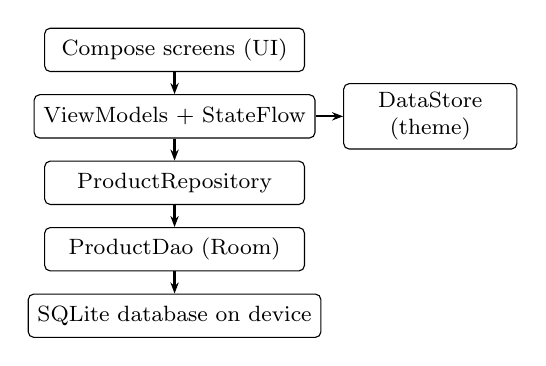
\begin{tikzpicture}[
  box/.style={draw, rounded corners=2pt, minimum width=3.3cm, minimum height=0.55cm,
              font=\footnotesize, align=center},
  arr/.style={-{Stealth[length=4pt]}, thick}]
  \node[box] (ui) {Compose screens (UI)};
  \node[box, below=0.28cm of ui] (vm) {ViewModels + StateFlow};
  \node[box, below=0.28cm of vm] (repo) {ProductRepository};
  \node[box, below=0.28cm of repo] (dao) {ProductDao (Room)};
  \node[box, below=0.28cm of dao] (db) {SQLite database on device};
  \node[box, right=0.35cm of vm, minimum width=2.2cm] (ds) {DataStore\\(theme)};
  \draw[arr] (ui) -- (vm); \draw[arr] (vm) -- (repo);
  \draw[arr] (repo) -- (dao); \draw[arr] (dao) -- (db);
  \draw[arr] (vm) -- (ds);
\end{tikzpicture}
\Description{Layered architecture: Compose UI, ViewModels, repository, Room DAO and SQLite; ViewModels also read DataStore.}
\caption{StockFlow architecture.}
\label{fig:arch}
\end{figure}

The single Room entity, \texttt{Product}, has an auto-generated integer key and
columns for name, SKU (unique index), category, color, size, description, quantity,
selling price, favorite flag and an optional image path. Table~\ref{tab:crud} maps
each CRUD operation to the user action that triggers it.

\begin{table}[h]
\caption{CRUD operations in StockFlow}
\label{tab:crud}
\footnotesize
\begin{tabular}{@{}l>{\raggedright\arraybackslash}p{3.1cm}>{\raggedright\arraybackslash}p{3.3cm}@{}}
\toprule
Operation & User action & DAO function \\
\midrule
Create & Save the Add Product form & \texttt{insertProduct} \\
Read & Home, Search, Favorites, Details & \texttt{getAllProducts}, \texttt{searchProducts}, \texttt{getProductById} \\
Update & Edit, favorite, Stock In/Out & \texttt{updateProduct} \\
Delete & Delete after confirmation & \texttt{deleteProduct} \\
\bottomrule
\end{tabular}
\end{table}

Stock Out is validated before any update: the requested amount must be a positive
whole number no larger than the current quantity, so stock can never become
negative. A chosen photo is copied into the app's private storage so that it stays
available after a restart. Product cards are laid out in an adaptive grid that shows
one column on phones and more on wider screens.

\section{Conclusion}
StockFlow delivers a focused, offline inventory tool for a clothing shop that covers
the Phase 1 requirements: Jetpack Compose screens connected by navigation, an
Android Intent for sharing, idiomatic Kotlin with lambdas and \texttt{val}/\texttt{var},
and complete CRUD on a persistent Room database. The layered design keeps each part
small enough for every team member to explain and leaves room to extend the app in
later phases.

\bibliographystyle{ACM-Reference-Format}
\bibliography{references}

\end{document}
